\documentclass[11pt]{article}
\usepackage{../../ee16}
\usepackage{../../markup}
\usepackage{tikz}
\usetikzlibrary{calc,shapes.geometric,arrows,automata}
\usepackage{color,hyperref,listings,enumitem}
\usepackage{algorithm}
\usepackage{algpseudocode}
\usepackage{tkz-euclide}
\usepackage{physics}
\usepackage{pgfplots}
\usepackage[american,siunitx]{circuitikz}
\usepackage{graphicx}
\lstset{basicstyle=\ttfamily}
\newcommand{\fillin}[1]{\underline{\hskip #1}}
\newcommand{\doublehrule}{\hrule \vskip 0.02in \hrule}
\newcommand*\circled[1]{\tikz[baseline=(char.base)]{
  \node[shape=circle,draw,inner sep=2pt] (char) {#1};}}

%\newcommand{\sol}[1]{{\color{blue} \textbf{Solution: } #1}} % solutions in blue
\newcommand{\sol}[1]{} % no solution sketches

%\newcommand{\ans}[1]{} % no numeric solutions
\newcommand{\ans}[1]{{\color{blueish} \textbf{Answer: } #1}} % numeric solutions

%\newcommand{\solans}[1]{}
\newcommand{\solans}[1]{{\color{blueish} \textbf{Answer: } #1}} %appears in both; use with caution

\begin{document}

\def\title{Worksheet 9}

\maketitle

\vspace{0.5em}

\begin{qunlist}
% Lydia Lee, lydia.lee@berkeley.edu
\qns{Live (And Die) By The Golden Rule(s)}

\sol{
	The purpose of this question is rote practice. While students will have seen many of these topologies, ask students if anyone wants things rederived.}
\begin{enumerate}
\qitem\label{golden_rules}
	What are the ``golden rules'' of op amps? Do any of them have conditions which must hold for them to be true?

	\begin{circuitikz}
		\draw (0,0) node[op amp,yscale=-1] (opamp) { }
		  (-2.5, 0.5) to [short, i=$i_{+}$, o-] (opamp.+) 
		  (-2.5, -0.5) to [short, i=$i_{-}$, o-] (opamp.-) 
		  (opamp.out) node[right ] {$U_{out}$} 
		  ;
		\node[draw=none,text=black] at (-2.8, 0.5) {$u_{+}$};
		\node[draw=none,text=black] at (-2.8, -0.5) {$u_{-}$};

		\draw (0, 0.5) to [short, -o] (0, 1.0);
		\node[draw=none,text=black] at (0, 1.5) {$V_{DD}$};
		\draw (0, -0.5) to [short, -o] (0, -1.0);
		\node[draw=none,text=black] at (0, -1.5) {$V_{SS}$};
	\end{circuitikz}

\ans{
	The Golden Rules of op amps with their necessary preconditions are:
	\begin{itemize}
		\item $i_+ = i_- = 0\si{\ampere}$. This is true of all op amps.
		\item When the op amp is in negative feedback, $u_+ = u_-$
	\end{itemize}}


\qitem\label{amplifier_topologies}
	For each of the following, find $v_\text{out}$ in terms of any input sources and any other given component values. First, solve for when $V_\text{REF} = 0\si{\volt}$. You may work out when $V_\text{REF} \neq 0\si{\volt}$ as a challenge. Assume the voltage rails are sufficient to not distort the output and that all op amps are in negative feedback. 
	\begin{enumerate}
		\item\label{buffer}\ \\
			\begin{circuitikz}[scale=0.8, transform shape]
	\draw
	(0,0) node[op amp,yscale=-1] (AMP) {}
	(AMP.-) to[short] ++(0,-1) coordinate (bottomLeft)
		to[short] (bottomLeft -| AMP.out)
		to[short] (AMP.out)
		to[short] ++(1,0)
		to[open,o-o,v^=$v_\text{out}$] ++(0,-2)
		node[ground] () {}
	(AMP.+) to[short,-o] ++(-2,0)
		node[anchor=east] () {$X$}
	;
\end{circuitikz}

			\sol{
				\begin{align*}
					v_\text{out} &= v_-\\
						&= v_+\\
						&= v_\text{in}
				\end{align*}}

			\ans{
				$v_\text{out} = v_\text{in}$}
		
		\item\label{buffer_res}\ \\
			\input{../../questionBank/week09/q_mech_nfb_figs/buffer_res}
			
			\sol{
				\begin{align*}
					v_\text{out} &= v_-\\
						&= v_+\\
						&= v_\text{in}
				\end{align*}}

			\ans{
				$v_\text{out} = v_\text{in}$. Remember that no current flows into the input terminals of the op amp!}

		\item\label{noninverting_amp}\ \\
			\begin{circuitikz}[scale=0.8, transform shape]
	\draw
	(0,0) node[op amp,yscale=-1] (AMP) {}
	(AMP.+) to[short,-o] ++(-2,0)
		node[anchor=east] () {$X$}
	(AMP.-) to[short] ++(0,-1.5) coordinate (bottomLeft)
		to[short] (bottomLeft -| AMP.out)
	(AMP.out) to[R,l_=$R_\text{top}$] (bottomLeft -| AMP.out)
		to[R,l_=$R_\text{bottom}$] ++(0,-1.5)
		to[V,l_=$V_\text{REF}$] ++(0,-1.5)
		node[ground] () {}
	(AMP.out) to[short] ++(1,0)
		to[open,o-o,v^=$v_\text{out}$] ++(0,-2)
		node[ground] () {}
	;
\end{circuitikz}

			\sol{
				\begin{align*}
					\frac{v_\text{out}-v_\text{in}}{R_\text{top}} &= \frac{v_\text{in}-V_\text{REF}}{R_\text{bottom}}\\
					v_\text{out} &= v_\text{in} + \frac{R_\text{top}}{R_\text{bottom}}\left(v_\text{in}-V_\text{REF}\right)\\
						&= v_\text{in}\left(1 + \frac{R_\text{top}}{R_\text{bottom}}\right) - V_\text{REF}\left(\frac{R_\text{top}}{R_\text{bottom}}\right)
				\end{align*}}

			\ans{
				$v_\text{out} = v_\text{in}\left(1 + \frac{R_\text{top}}{R_\text{bottom}}\right) - V_\text{REF}\left(\frac{R_\text{top}}{R_\text{bottom}}\right)$}

		\item\label{inverting_amp}\textit{Hint: Is this similar at all to part \ref{noninverting_amp}?}\\
			\begin{circuitikz}[scale=0.8, transform shape]
	\draw
	(0,0) node[op amp] (AMP) {}
	(AMP.-) to[short] ++(0,1) coordinate (topLeft)
		to[R,l=$R_f$] (topLeft -| AMP.out)
		to[short] (AMP.out)
		to[short,-o] ++(1,0)
		to[open,o-o,v^=$v_\text{out}$] ++(0,-2)
		node[ground] () {}
	(AMP.-) to[R,l_=$R_s$,-o] ++(-2,0)
		node[anchor=east] () {$X$}
	(AMP.+) to[V,l_=$V_\text{REF}$] ++(0,-2)
		node[ground] () {};
\end{circuitikz}

			\sol{
				\begin{align*}
					\frac{v_\text{in}-V_\text{REF}}{R_s} &= \frac{V_\text{REF}-v_\text{out}}{R_f}\\
					V_\text{REF}-v_\text{out} &= \frac{R_f}{R_s}\left(v_\text{in}-V_\text{REF}\right)\\
					v_\text{out} &= V_\text{REF}\left(1 + \frac{R_f}{R_s}\right) - v_\text{in}\left(\frac{R_f}{R_s}\right)
				\end{align*}}

			\ans{
				$v_\text{out} = v_\text{in}\left(-\frac{R_f}{R_s}\right) + V_\text{REF}\left(\frac{R_f}{R_s} + 1\right)$. Note that this is exactly the same as \ref{noninverting_amp} with $v_\text{in}$ and $V_\text{REF}$ switched!}

		\item\label{inverting_summing_amp}\ \\
			\begin{circuitikz}[scale=0.8, transform shape]
	\draw
	(0,0) node[op amp] (AMP) {}
	(AMP.-) to[short] ++(0,1) coordinate (topLeft)
		to[R,l=$R_f$] (topLeft -| AMP.out)
		to[short] (AMP.out)
		to[short,-o] ++(1,0)
		to[open,o-o,v^=$v_\text{out}$] ++(0,-2)
		node[ground] () {}
	(AMP.-) to[short] ++(-.5,0) coordinate (summing)
		to[R,l_=$R_{s1}$] ++(-2,0)
		to[/tikz/circuitikz/bipoles/length=1cm,sV,v_=$v_\text{in1}$] ++(0,-1)
		node[ground] () {}
	(summing) to[short] ++(0,2)
		to[R,l_=$R_{s2}$] ++(-2,0)
		to[/tikz/circuitikz/bipoles/length=1cm,sV,v_=$v_\text{in2}$] ++(0,-1)
		node[ground] () {}
	(AMP.+) to[V,l_=$V_\text{REF}$] ++(0,-2)
		node[ground] () {};
\end{circuitikz}
			
			\sol{
				\textbf{KCL}: There are a few ways to do this, but the fastest way is through KCL, a.k.a. nodal analysis
				\begin{align*}
					\frac{v_\text{in1}-V_\text{REF}}{R_{s1}} + \frac{v_\text{in2}-V_\text{REF}}{R_{s2}} &= \frac{V_\text{REF}-v_\text{out}}{R_f}\\
					V_\text{REF}-v_\text{out} &= R_f\left(\frac{v_\text{in1}}{R_{s1}} + \frac{v_\text{in2}}{R_{s2}} - V_\text{REF}\left(\frac{1}{R_{s1}} + \frac{1}{R_{s2}}\right)\right)\\
					v_\text{out} &= v_\text{in1}\left(\frac{-R_f}{R_{s1}}\right) + v_\text{in2}\left(\frac{-R_f}{R_{s2}}\right) + V_\text{REF}\left(\frac{R_f}{R_{s1}} + \frac{R_f}{R_{s2}} + 1\right)
				\end{align*}
				\textbf{Superposition}: As with all circuit problems, this can also be solved via superposition. Turning off all independent sources but $v_\text{in1}$, $v_\text{in2}$, and $V_\text{REF}$ in order:
				\begin{align*}
					\frac{v_\text{in1}}{R_{s1}} &= \frac{0-v_\text{out1}}{R_f}\\
					v_\text{out1} &= v_\text{in1}\left(-\frac{R_f}{R_{s1}}\right)\\
				\end{align*}
				Finding the effect of $v_\text{in2}$ is identical to the process used for $v_\text{in1}$
				\begin{align*}
					\frac{v_\text{in2}}{R_{s2}} &= \frac{0-v_\text{out2}}{R_f}\\
					v_\text{out2} &= v_\text{in2}\left(-\frac{R_f}{R_{s2}}\right)\\
				\end{align*}
				With just $V_\text{REF}$ on and the other two independent voltages sources turned off, we see a noninverting amplifier.
				\begin{align*}
					V_\text{REF} &= v_\text{out,REF}\frac{R_{s1}||R_{s2}}{R_f + R_{s1}||R_{s2}}\\
					v_\text{out,REF} &= V_\text{REF}\left(1 + \frac{R_f}{R_{s1}||R_{s2}}\right)
				\end{align*}
				And adding all of the results together:
				\begin{align*}
					v_\text{out} &= v_\text{out1} + v_\text{out2} + v_\text{outREF}\\
						&= v_\text{in1}\left(-\frac{R_f}{R_{s1}}\right) + v_\text{in2}\left(-\frac{R_f}{R_{s2}}\right) + V_\text{REF}\left(1 + \frac{R_f}{R_{s1}||R_{s2}}\right)
				\end{align*}}

			\ans{
				\begin{align*}
					v_\text{out} &= v_\text{in1}\left(\frac{-R_f}{R_{s1}}\right) + v_\text{in2}\left(\frac{-R_f}{R_{s2}}\right) + V_\text{REF}\left(\frac{R_f}{R_{s1}} + \frac{R_f}{R_{s2}} + 1\right)\\
						&= v_\text{in1}\left(-\frac{R_f}{R_{s1}}\right) + v_\text{in2}\left(-\frac{R_f}{R_{s2}}\right) + V_\text{REF}\left(1 + \frac{R_f}{R_{s1}||R_{s2}}\right)
				\end{align*}}

		\item\label{transimpedance_amp}\ \\
			\input{../../questionBank/week09/q_mech_nfb_figs/transimpedance_amp}

			\sol{
				\begin{align*}
					i_\text{in} &= \frac{V_\text{REF}-v_\text{out}}{R}\\
					v_\text{out} &= V_\text{REF}-i_\text{in}R
				\end{align*}}

			\ans{
				$v_\text{out} = i_\text{in}(-R) + V_\text{REF}$}
		
		\item\label{integrator_voltage}Assume you know $v_\text{out}(t_0)$.\\
			\begin{circuitikz}[scale=0.8, transform shape]
	\draw
	(0,0) node[op amp] (AMP) {}
	(AMP.out) to[short] ++(0,2) coordinate (topRight)
		to[C,l_=$C$] (topRight -| AMP.-)
		to[short] (AMP.-)
		to[R,l_=$R$] ++(-2,0)
		to[sV,v_=$v_\text{in}$] ++(0,-2) coordinate (groundPlane)
		node[ground] () {}
	(AMP.+) to[short] ++(-.5,0) coordinate
		to[V,v=$V_\text{REF}$] ++(0,-2)
		node[ground] () {}
	(AMP.out) to[short] ++(1,0) coordinate (outOut)
		to[open,o-o,v^=$v_\text{out}$] (outOut |- groundPlane)
		node[ground] () {};
\end{circuitikz}
			
			\sol{
				\begin{align*}
					\frac{v_\text{in}-V_\text{REF}}{R} &= C\frac{d(V_\text{REF}-v_\text{out})}{dt}\\
						&= C\left(\frac{dV_\text{REF}}{dt} - \frac{dv_\text{out}}{dt}\right)\\
						&= -C\frac{dv_\text{out}}{dt} \longleftarrow \frac{dV_\text{REF}}{dt} = 0\\
					\frac{dv_\text{out}}{dt} &= -\frac{1}{RC}(v_\text{in}-V_\text{REF})\\
					v_\text{out}(t) - v_\text{out}(t_0) &= \int_{t_0}^t-\frac{v_\text{in}-V_\text{REF}}{RC}d\tau\\
					v_\text{out}(t) &= v_\text{out}(t_0) + \int_{t_0}^t\frac{V_\text{REF}-v_\text{in}}{RC}d\tau
				\end{align*}}

			\ans{
				$v_\text{out}(t) = v_\text{out}(t_0) + \int_{t_0}^t\frac{V_\text{REF}-v_\text{in}}{RC}d\tau$. Note that your voltages may not be constant with respect to time!}
		\empt{\newpage}
		\item\label{differentiator}\textbf{(PRACTICE)}\\
			\begin{circuitikz}[scale=0.8, transform shape]
	\draw (0,0) node[op amp] (AMP) {}
        (AMP.out) to[short] ++(0,2) coordinate (topRight)
        to[R,l_=$R$] (topRight -| AMP.-)
        to[short] (AMP.-)
        to[C,l_=$C$] ++(-2,0)
        to[sV,v_=$v_\text{in}$] ++(0,-2)
        node[ground] () {}
    (AMP.+) to[short] ++(-.5,0)
        to[V,v=$V_\text{REF}$] ++(0,-2)
        node[ground] () {}
    (AMP.out) to[short] ++(1,0)
        to[open,v^=$v_\text{out}$,o-o] ++(0,-2)
        node[ground] () {};
\end{circuitikz}

			\sol{
				\begin{align*}
					\frac{V_\text{REF}-v_\text{out}}{R} &= C\frac{d(v_\text{in}-V_\text{REF})}{dt}\\
						&= C\left(\frac{d(v_\text{in}}{dt}-\frac{V_\text{REF})}{dt}\right)\\
					v_\text{out} &= V_\text{REF} - RC\frac{dv_\text{in}}{dt} \longleftarrow \frac{dV_\text{REF}}{dt} = 0
				\end{align*}}

			\ans{
				$v_\text{out} = V_\text{REF} - RC\frac{dv_\text{in}}{dt}$}
		
		% \item\label{instrumentation_amp}\textbf{(CHALLENGE PRACTICE)}\\
		% 	\begin{circuitikz}[scale=0.8, transform shape]
	\draw
	(0,0) node[op amp,yscale=-1] (AMP_TOP) {}
	(0,-6) node[op amp] (AMP_BOT) {}
	(5,-3) node[op amp] (AMP_OUT) {}

	% Input voltage sources
	(AMP_TOP.+) to[short] ++(-1,0)
		to[sV,v_=$v_\text{in1}$] ++(0,-2)
		node[ground] () {}

	(AMP_BOT.+) to[short] ++(-1,0)
		to[sV,v_=$v_\text{in2}$] ++(0,-2)
		node[ground] () {}

	% First layer of resistors
	(AMP_TOP.-) to[short] ++(0,-1.5) coordinate (topMinusExtension)
		to[short] (topMinusExtension -| AMP_TOP.out)
		to[R=$R_1$] (AMP_TOP.out)
	(AMP_BOT.-) to[short] ++(0,1.5) coordinate (botMinusExtension)
		to[short] (botMinusExtension -| AMP_BOT.out)
		to[R=$R_1$] (AMP_BOT.out)
	(topMinusExtension -| AMP_TOP.out) to[R=$R_{\text{gain}}$] (botMinusExtension -| AMP_BOT.out)

	% Second layer of resistors
	(AMP_TOP.out) to[R=$R_2$] (AMP_TOP.out -| AMP_OUT.-)
		to[short] (AMP_OUT.-)
	(AMP_BOT.out) to[R=$R_2$] (AMP_BOT.out -| AMP_OUT.+)
		to[short] (AMP_OUT.+)

	% Third layer of resistors
	(AMP_OUT.out) to[short] (AMP_OUT.out |- AMP_TOP.out)
		to[R=$R_3$] (AMP_TOP.out -| AMP_OUT.-)
		to[short] (AMP_OUT.-)
	(AMP_OUT.+) to[short] (AMP_OUT.+ |- AMP_BOT.out)
		to[R=$R_3$] (AMP_BOT.out -| AMP_OUT.out)
		node[ground] () {}
	
	% Final output
	(AMP_OUT.out) to[short] ++(1,0)
		to[open,o-o,v^=$v_\text{out}$] ++(0,-3)
		node[ground] () {}
	;
\end{circuitikz}
	\end{enumerate}


\end{enumerate}
% Lydia Lee, lydia.lee@berkeley.edu
\qns{Loaded Question}

\begin{enumerate}

\qitem\label{rin}{
	Assume you're given the following block:
	\begin{center}
		\begin{circuitikz}[scale=0.75, transform shape]
			\draw
			(0,0) node[ground] () {}
				to[sV,l=$v_S$] ++(0,3)
				to[short] ++(1,0)
				to[R=$R_\text{top}$] ++(0,-1.5) coordinate (output)
				to[R=$R_\text{bottom}$] ++(0,-1.5)
				node[ground] () {}

			(output) to[short,*-] ++(2,0)
				node[anchor=south] () {$X$}
				to[open,o-o,v^=$v_X$] ++(0,-1.5)
				node[ground] () {};
		\end{circuitikz}
	\end{center}
	For each of the following, replace the input voltage source with the circuit above. For the full circuit, is the value of $v_X$ affected by the attachment of the second block, i.e. does it load the voltage divider?

	\begin{enumerate}
		\item \ \\
		\begin{circuitikz}[scale=0.75, transform shape]
			\draw
			(0,0) node[ground] () {} 
				to[sV,l=$v_\text{in}$] ++(0,1.5)
				to[short] ++(1.5,0)
				to[R=$R_L$] ++(0,-1.5)
				node[ground] () {};
		\end{circuitikz}
		\item \ \\
			\begin{circuitikz}[scale=0.8, transform shape]
	\draw
	(0,0) node[op amp,yscale=-1] (AMP) {}
	(AMP.-) to[short] ++(0,-1) coordinate (bottomLeft)
		to[short] (bottomLeft -| AMP.out)
		to[short] (AMP.out)
		to[short] ++(1,0)
		to[open,o-o,v^=$v_\text{out}$] ++(0,-2)
		node[ground] () {}
	(AMP.+) to[short,-o] ++(-2,0)
		node[anchor=east] () {$X$}
	;
\end{circuitikz}
		\item \ \\
			\begin{circuitikz}[scale=0.8, transform shape]
	\draw
	(0,0) node[op amp,yscale=-1] (AMP) {}
	(AMP.+) to[short,-o] ++(-2,0)
		node[anchor=east] () {$X$}
	(AMP.-) to[short] ++(0,-1.5) coordinate (bottomLeft)
		to[short] (bottomLeft -| AMP.out)
	(AMP.out) to[R,l_=$R_\text{top}$] (bottomLeft -| AMP.out)
		to[R,l_=$R_\text{bottom}$] ++(0,-1.5)
		to[V,l_=$V_\text{REF}$] ++(0,-1.5)
		node[ground] () {}
	(AMP.out) to[short] ++(1,0)
		to[open,o-o,v^=$v_\text{out}$] ++(0,-2)
		node[ground] () {}
	;
\end{circuitikz}
		\item \ \\
			\begin{circuitikz}[scale=0.8, transform shape]
	\draw
	(0,0) node[op amp] (AMP) {}
	(AMP.-) to[short] ++(0,1) coordinate (topLeft)
		to[R,l=$R_f$] (topLeft -| AMP.out)
		to[short] (AMP.out)
		to[short,-o] ++(1,0)
		to[open,o-o,v^=$v_\text{out}$] ++(0,-2)
		node[ground] () {}
	(AMP.-) to[R,l_=$R_s$,-o] ++(-2,0)
		node[anchor=east] () {$X$}
	(AMP.+) to[V,l_=$V_\text{REF}$] ++(0,-2)
		node[ground] () {};
\end{circuitikz}
	\end{enumerate}
	}

\sol{
	What this is asking for can be written in a few equivalent ways:
	\begin{itemize}
		\item Is the Th\'evenin resistance ($R_{\text{in}}$) from the input node of the circuit finite?
		\item Will the circuit in question load the voltage divider above?
		\item Does the circuit draw current from its input node?
	\end{itemize}
	FINISH THIS!!! - this section should have (1) the full circuit analysis (2) the computation finding the input resistance of the circuit.
	\begin{enumerate}
		\item 
		\item
		\item
	\end{enumerate}
}

\ans{
	\begin{enumerate}
		\item This is a voltage buffer! It does not affect the value of $v_x$ of the voltage divider.
		\item This is a noninverting amplifier. Note that no current is drawn from the voltage source because $i_+ = i_- = 0\si{\ampere}$; that said, it does not load the voltage follower and so does not affect the value of $v_X$ from its original value.
		\item This is an inverting amplifier. In this case, current flows across $R_s$, meaning that the amplifier \textit{does} in fact load the voltage divider and affects the value of $v_X$!
	\end{enumerate}
}

\qitem\label{rout}{
	For the following blocks, determine if attaching $R_L$ between the output and ground affects $v_\text{out}$
	\begin{enumerate}
		\item \ \\
			\input{../../questionBank/week09/q_loading_figs/buffer_ro}
		\item \ \\
			\input{../../questionBank/week09/q_loading_figs/inverting_amp_ro}
		\item \ \\
			\input{../../questionBank/week09/q_loading_figs/buffer_rl_series}
		\item \ \\
			\input{../../questionBank/week09/q_loading_figs/inverting_amp_rl_parallel}
	\end{enumerate}
}

\sol{
	After enough practice, students should be able to do these types of problems by inspection. Poll your class if they think yes/no. If students ask, you should be ready to work out the full solution.}

\ans{
	\begin{enumerate}
		\item The configuration shown in this part is a voltage buffer. Attaching $R_L$ between output and ground won't affect $v_{out}$ because the output voltage remains the same across nodes.
		\item As shown, we essentially have an inverting amplifier for this configuration. However, $r_{\rho}$ is within the output node of the amplifier, attaching $R_L$ will have the same effect as in the previous part. The output voltage still remains the same.
		\item Since we connect $r_o$ outside the output of the amplifier, once we attach $R_L$ between the end node and the ground, we have essentially built a voltage divider with the 2 resistors, which decreases the output voltage!
		\item For this circuit, when we attach $R_L$ between the output and the ground, we can see that $r_l$ and $R_L$ are both in parallel, and the positive end of $v_out$ can be seen directly connected to the output node of the amplifier, which isn't affected by any resistor(s) along the way. Hence, the output voltage won't change.
	\end{enumerate}
}
\end{enumerate}
\empt{\newpage}
% Lydia Lee, lydia.lee@berkeley.edu
\qns{\textbf{(EXAM-STYLE PRACTICE)} Automatic Gain Control}

\sol{This is a design problem meant to be there \textbf{only if} students ask for exam-style practice, and as such it goes a bit beyond the standard mechanical practice/solidifying basics style CSM tends to offer. For useful amplifier topologies, see \lstinline{q_mech_nfb.tex}}

\begin{enumerate}
\qitem\label{amp}{
	Design a circuit where $V_\text{out} = -10V_\text{in}$. You are allowed to use
	\begin{itemize}
		\item op amps: $\leq$1. You do not need to specify rail voltages for this subpart.
		\item resistors: as many as you want, so long as they have positive values
		\item capacitors: as many as you want
	\end{itemize}}

\empt{
	\vspace{1cm}
	\begin{circuitikz}
		\draw
		(0,0) to[short] ++(-1,0)
			to[sV,v_=$V_\text{in}$] ++(0,-2)
			node[ground] () {};
	\end{circuitikz}
	\vspace{1cm}}

\ans{
	This is one possible solution:
	\begin{center}
		\begin{circuitikz}[scale=0.8, transform shape]
	\draw
	(0,0) node[op amp] (AMP) {}
	(AMP.-) to[short] ++(0,1) coordinate (topLeft)
		to[R,l=$10R$] (topLeft -| AMP.out)
		to[short] (AMP.out)
		to[short,-o] ++(1,0)
		to[open,o-o,v^=$V_\text{out}$] ++(0,-2)
		node[ground] () {}
	(AMP.-) to[R,l_=$R$] ++(-2,0)
		to[sV,v_=$V_\text{in}$] ++(0,-2)
		node[ground] () {}
	(AMP.+) to[short] ++(0,-1)
		node[ground] () {};
\end{circuitikz}
	\end{center}}

\qitem\label{no_rail}{
	Your design was provided voltage rails at $5\si{\volt}$ and $-5\si{\volt}$, and that your input signal looks like so:
	\begin{center}
		\input{../../questionBank/week09/q_design_agc_figs/no_rail_input}
	\end{center}
	Will your signal be faithfully amplified when $V_\text{out} = -10V_\text{in}$, or will it rail/clip?}

\empt{\vspace{1.5cm}}

\ans{
	The signal will be faithfully amplified.

	Our output is going to be limited to $\pm 5\si{\volt}$, meaning that with an amplifier gain $\frac{V_\text{out}}{V_\text{in}} = 10$, we can have an input no larger than $0.5\si{\volt}$ in the positive or negative direction.}

\qitem\label{yes_rail}{
	Again, your design has voltage rails at $\pm 5\si{\volt}$. Your input signal now looks like so:
	\begin{center}
		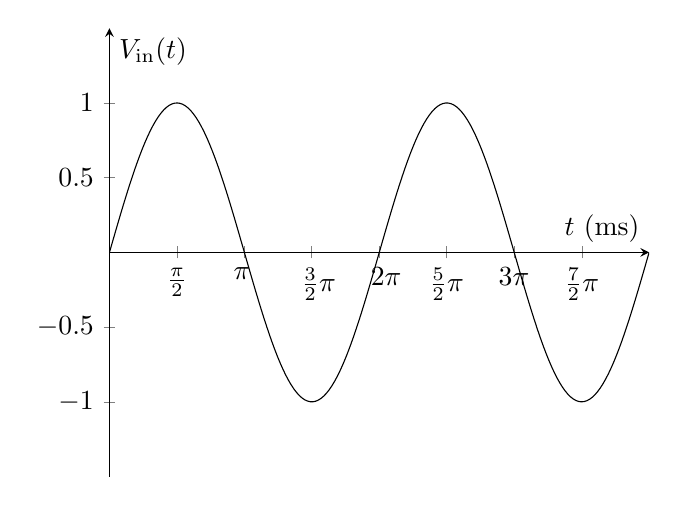
\begin{tikzpicture}
\begin{axis}[
    axis lines = middle,
    xlabel = {$t$ $(\si{\milli\second})$},
    ylabel = {$V_\text{in}(t)$},
    xtick={0,1.57,3.14,4.71,6.28, 7.85, 9.42, 11.00, 12.57},
    xticklabels={$0$, $\frac{\pi}{2}$,$\pi\,$,$\,\,\,\frac{3}{2}\pi$,$\,\,\,2\pi$, $\frac{5}{2}\pi$, $3\pi$, $\frac{7}{2}\pi$, $4\pi$},
    ytick={0,-0.5,0.5,-1,1},
    ymin=-1.5,
    ymax=1.5,
    xmin = 0,
    xmax=4*pi
]
\addplot [
	color=black,
	domain=0:4*pi,
	samples=200
	]
	{ sin(deg(x))  
	};
\end{axis}
\end{tikzpicture}
	\end{center}
	With this input signal and $V_\text{out} = -10V_\text{in}$, will your amplifier  distort the output due to railing/clipping?}

\empt{\vspace{1.5cm}}

\ans{
	The output will experience railing. From the explanation for part \ref{no_rail}, we know our input can swing no further than $0.5\si{\volt}$, and in this case the swing is $1\si{\volt}$.}

\qitem\label{resistorDAC}{
	Design a circuit which can have a resistance $R$ when an input signal $\phi$ is high and a resistance $nR$ ($n > 1$) when $\phi$ is low. You have access to:
	\begin{itemize}
		\item ideal switches: as many as you want
		\item resistors with positive values: $\leq 2$
		\item the signal $\phi$ and its complement, $\overline{\phi}$
	\end{itemize}}

\empt{\vspace{4cm}}

\ans{
	One possible solution is to place the resistor in series and short it out when $\phi$ is high:
	\begin{center}
		\begin{circuitikz}[scale=0.8, transform shape]
	\draw
	(0,0) to[short,o-] ++(1,0) coordinate (leftSide) 
		to[R=$(n-1)R$] ++(2,0) coordinate(rightSide)
		to[R=$R$] ++(2,0)
		to[short,-o] ++(1,0)
	(leftSide) to[short] ++(0,1.5) coordinate (topLeft)
		to[spst,l=$\phi$] (topLeft -| rightSide)
		to[short] (rightSide);
\end{circuitikz}
	\end{center}

	Another possible solution is to place the resistor in parallel and place a switch in series with it to close whenever $\phi$ is high. Remember that in parallel, the resistance decreases!
	\begin{center}
		\begin{circuitikz}[scale=0.8, transform shape]
	\draw
	(0,0) to[short,o-] ++(1,0) coordinate (leftSide)
		to[R=$nR$] ++(4,0) coordinate (rightSide)
		to[short,-o] ++(1,0)
	(leftSide) to[short] ++(0,1.5)
		to[spst,l=$\phi$] ++(2,0)
		to[R=$R\left(\frac{n}{n-1}\right)$] ++(2,0)
		to[short] (rightSide);
\end{circuitikz}
	\end{center}}

\qitem\label{vga}{
	Using your answer from parts \ref{amp} and \ref{resistorDAC}, design a circuit where
	$$V_\text{out} = \begin{cases}
						-5V_\text{in} & \phi = \text{high}\\
						-10V_\text{in} & \phi = \text{low}
					\end{cases}$$}
\empt{
	\vspace{1cm}
	\begin{circuitikz}
		\draw
		(0,0) to[short] ++(-1,0)
			to[sV,v_=$V_\text{in}$] ++(0,-2)
			node[ground] () {};
	\end{circuitikz}
	\vspace{1cm}}

\ans{
	Using the symbol for a variable resistor,
	\begin{center}
		\input{../../questionBank/week09/q_design_agc_figs/sol_vga}
	\end{center}
	we can replace $R_\text{var}$ with our answer to part \ref{resistorDAC}.
}

\qitem\label{phi_oneSide}{
	How do we generate $\phi$? We want it to be high whenever $|V_\text{in}|$ is larger than some threshold, and low otherwise. Before jumping to absolute value, let's look at a slightly simpler problem: design a circuit whose output is
	$$\phi_\text{high-side} = \begin{cases}
								V_{DD} & V_\text{in} < -0.49\si{\volt}\\
								V_{SS} & V_\text{in} > -0.49\si{\volt}
							\end{cases}$$
	You may use:
	\begin{itemize}
		\item op amps: as many as you want
		\item ideal voltage source: $\leq 1$ in addition to the $\pm 5\si{\volt}$ voltage rails
		\item your answer to part \ref{amp}, black-boxed to take in $V_\text{in}$. You may assume it works as described in part \ref{amp}
	\end{itemize}}

\empt{
	\vspace{1cm}
	\begin{circuitikz}
		\draw
		(0,0) to[short] ++(-2,0)
			to[sV,v_=$V_\text{in}$] ++(0,-2)
			node[ground] () {};
	\end{circuitikz}
	\vspace{1cm}}


\ans{
	One possible solution:
	\begin{center}
		\begin{circuitikz}[scale=0.8, transform shape]
	\draw
	(0,0) node[op amp] (AMP) {}
	(4,-0.5) node[op amp,yscale=-1] (COMP) {}

	(AMP.-) to[short] ++(0,1) coordinate (topLeft)
		to[R,l=$10R$] (topLeft -| AMP.out)
		to[short] (AMP.out)
		to[short] (COMP.+)
	(AMP.-) to[R,l_=$R$] ++(-2,0)
		to[sV,v_=$V_\text{in}$] ++(0,-2)
		node[ground] () {}
	(AMP.+) to[short] ++(0,-1)
		node[ground] () {}
	(COMP.-) to[V=$4.9\si{\volt}$] ++(0,-2)
		node[ground] () {}
	(COMP.out) to[short,-o] ++(1,0)
		node[anchor=west] () {$\phi_\text{high-side}$};
\end{circuitikz}
	\end{center}

	Mind your polarity! Remember that part \ref{amp} has a negative relationship between its output and $V_\text{in}$.
}

\qitem\label{agc}{
	Now let's put it all together. Design a circuit which lowers the gain setting when the input swing exceeds $0.49\si{\volt}$ (we usually like to leave some wriggle room just in case). You may assume all feedback loops are infinitely fast.
	$$V_\text{out} = \begin{cases}
						-5V_\text{in} & |V_\text{in}| > 0.49\si{\volt}\\
						-10V_\text{in} & |V_\text{in}| < 0.49\si{\volt}
					\end{cases}$$
	You may use
	\begin{itemize}
		\item op amps: as many as you want
		\item switches: as many as you want
		\item resistors with positive values: as many as you want
		\item ideal voltage source: $\leq 2$, in addition to the provided rails $\pm 5\si{\volt}$
		\item your answer to part \ref{vga}, black-boxed to take in $V_\text{in}$ and $\phi$. You may assume it works as described in part \ref{vga}.
		\item a device which returns the maximum of its two inputs: $\leq 1$
		\begin{center}
			\begin{circuitikz}
				\draw (0,0) node[or port] (OR) {}
				(OR.in 1) node[anchor=east] () {$V_\text{in1}$}
				(OR.in 2) node[anchor=east] () {$V_\text{in2}$}
				(OR.out) node[anchor=west] () {$V_\text{max}$};
			\end{circuitikz}
		\end{center}
	\end{itemize}
	\textit{Hint: It may be helpful to consider the single-sided case when $V_\text{in} > 0.49\si{\volt}$ first, then only start worrying about the negative case $V_\text{in} < -0.49\si{\volt}$ afterward.}}
	

\empt{
	\vspace{3cm}
	\begin{circuitikz}
		\draw
		(0,0) to[short] ++(-1,0)
			to[sV,v_=$V_\text{in}$] ++(0,-2)
			node[ground] () {};
	\end{circuitikz}}

\sol{
	This may be a large jump for your students. If they're stumped, try prompting them in this order:
	\begin{enumerate}
		\item What component generates a high or low voltage depending on which input is larger/smaller? (Almost like we're going to \textit{compare} the inputs)
		\item What would we do if we only wanted to change the gain setting when $V_\text{in} > 0.49\si{\volt}$ and not worry about the negative case?
		\item How about the negative-only case, i.e. when $V_\text{in} < -0.49\si{\volt}$?
		\item How can we combine these?
	\end{enumerate}}

\ans{
	One possible solution:
	\begin{center}
		\begin{circuitikz}[scale=0.8, transform shape]
	\draw
	(0,0) node[op amp] (AMP) {}
	(5,-2.5) node[op amp,yscale=-1] (COMP_HI) {}
	(5,2.5) node[op amp] (COMP_LO) {}
	(9,0) node[or port] (OR) {}
	(AMP.-) to[short] ++(0,1) coordinate (topLeft)
		to[vR,l=$R_\text{var}$] (topLeft -| AMP.out)
		to[short] (AMP.out)
		to[short,-o] ++(1,0) coordinate (connector)
		node[anchor=west] () {$V_\text{out}$}
	(AMP.-) to[R,l_=$R$] ++(-2,0)
		to[sV,v_=$V_\text{in}$] ++(0,-2)
		node[ground] () {}
	(AMP.+) to[short] ++(0,-1)
		node[ground] () {}
	(COMP_HI.+) to[short] ++(-1,0)
		node[anchor=east] () {$V_\text{in}$}
	(COMP_LO.-) to[short] ++(-1,0)
		node[anchor=east] () {$V_\text{in}$}
	(COMP_HI.-) to[V=$0.49\si{\volt}$] ++(0,-2)
		node[ground] () {}
	(COMP_LO.+) to[V=$-0.49\si{\volt}$] ++(0,-2)
		node[ground] () {}
	(COMP_HI.out) to[short] (COMP_HI.out |- OR.in 2)
		to[short] (OR.in 2)
	(COMP_LO.out) to[short] (COMP_LO.out |- OR.in 1)
		to[short] (OR.in 1)
	(OR.out) node[anchor=west] () {$\phi$};
\end{circuitikz}
	\end{center}
	Note that this solution is aggressive and minimal.}
\end{enumerate}

\empt{\newpage}
\input{../../questionBank/week11/q_modular_circuits}
\end{qunlist}

\end{document}

